\documentclass[11pt]{amsart}

\usepackage{a4wide}
\usepackage{paralist}
\usepackage{url}
\usepackage{nopageno}
\usepackage{graphicx}

\newcommand{\cA}{\mathcal{A}}
\newcommand{\cS}{\mathcal{S}}
\newcommand{\N}{\mathbb{N}}
\newcommand{\Q}{\mathbb{Q}}
\newcommand{\R}{\mathbb{R}}
\newcommand{\Z}{\mathbb{Z}}


\begin{document}
\begin{center}
\textbf{\sffamily
   Discrete and Algorithmic Geometry }

\medskip
   Julian Pfeifle,
   UPC, 2013 \mbox{}
\end{center}

\bigskip

\begin{center}
  \textbf{\sffamily Sheet 2}

\bigskip
%\textbf{\sffamily UNDER CONSTRUCTION}
 due on Monday, November 18, 2013

\end{center}

%\bigskip
%\bigskip
\bigskip
\enlargethispage{2cm}
\section*{Reading}

\begin{enumerate}
\setlength{\itemsep}{2ex}
\item Read Lectures 3, 4 from Ziegler's \emph{Lectures on Polytopes}.

%\item Read Sections 5.1, 5.2, 5.3 from Matou\v sek's \emph{Lectures on
%    Discrete Geometry}.
\end{enumerate}

%\bigskip
%\bigskip
\section*{Writing}

\begin{enumerate}

\item Show that a face $F$ of a polytope $P$ is exactly the convex hull of all vertices of $P$ contained in~$F$. 
In particular, $P$~has only finitely many faces.

\item Let $P\subset\R^d$, $Q\subset\R^e$ be two non-empty polytopes. Prove that the set of faces of the cartesian product polytope $P\times Q=\{(p,q)\in\R^{d+e}:p\in P,\; q\in Q\}$ exactly equals $\{F\times G: F\text{ is face of }P, \;G\text{ is face of }Q\}$. Conclude that
\[
    f_k(P\times Q)
    \ = \
    \sum_{%\substack{
      i+j=k,\;i,j\ge0}f_i(P) f_j(Q)
    \qquad
    \text{for } k\ge0.
\]

\item Show that all induced cycles of length $3$, $4$ and $5$ in the graph of a simple $d$-polytope~$P$ are graphs of $2$-faces of $P$.
Conclude that the Petersen graph is not the graph of any polytope of any dimension. (\emph{Hint for $5$-cycles:} First show this for $d=3$. Then prove
that any $5$-cycle in a simple polytope is contained in some $3$-face,
and use that faces of  simple polytopes are simple.)

\item Let $n\in\N$ be an integer and $S$ denote a subset of
  $\{1,2,\dots,\lfloor\frac{n}{2}\rfloor\}$.  
  The \emph{circulant graph} $\Gamma_n(S)$ is the graph whose vertex set is $\Z_n$, and whose edge set is the set of pairs of vertices whose difference lies in $S\cup (-S)$. 

The following figure collects all connected circulant graphs on up to $8$~vertices. Determine the \emph{polytopality range} for as many of these graphs as you can, i.e., the set of integers~$d$ such that the graph in question is the graph of a $d$-dimensional polytope.

\bigskip
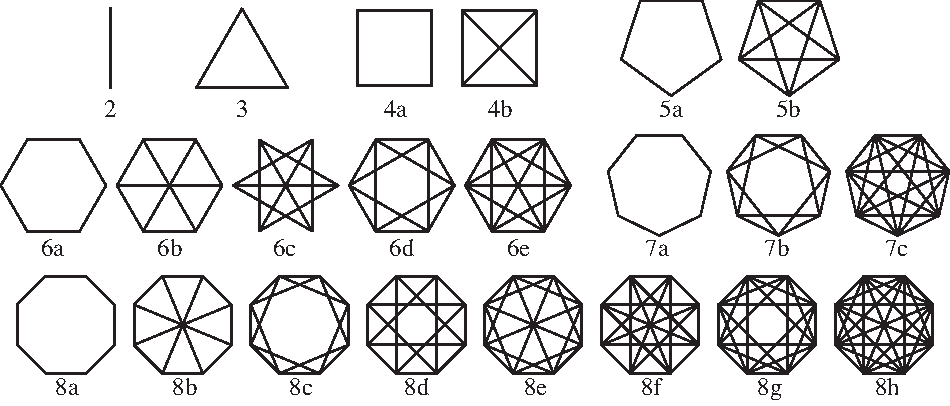
\includegraphics[width=\linewidth]{circulant}

\item Let $\Box^d$ be the $d$-dimensional $\pm1$-cube. How large can the volume of a simplex in $\Box^d$ become? (\emph{Hint:} \url{en.wikipedia.org/wiki/Hadamard_inequality}. Write a  C++ program to attain explicit bounds for $d\ge2$ as large as you can.)
\end{enumerate}

% \bigskip
% \bigskip
% \section*{Software}

% \begin{enumerate}
% \setlength{\itemsep}{2ex}
% \item
% \end{enumerate}

\end{document}
